\def\Ponderation{35}
\def\SigleNumero{STT-1000}
\def\NomCours{Probabilités et statstique}
\def\DateEvaluation{8 janvier 2026}
\def\HeureEvaluation{}
\def\Session{}
\def\NomEvaluation{Examen 1}
\def\Ponderation{35}
% Ne rien mettre entre les accolades si l'enseignant (ou l'enseignante) est aussi le coordonnateur (ou la coordonnatrice)
\def\Coordonnatrice{}
\def\Coordonnateur{}

% Ne rien mettre entre les accolades s'il y a plus d'une section
\def\Enseignant{}
\def\Enseignante{}

% Ne rien mettre entre les accolades s'il s'agit d'un cours à section unique
% Mettre le nom de chacun des enseignants et enseignantes entre les accolades
% Une case à cocher sera générée pour chacune des sections
\def\SectionA{Ahmed Sid-Ali}
\def\SectionB{Julien Miron}
\def\SectionC{}
\def\SectionD{}


\def\Directives{
\begin{enumerate}
\item Matériel autorisé:
\begin{itemize}
\item Calculatrice scientifique {\bf autorisée par la faculté des sciences et de génie};
\item Le feuillet de formules fourni avec l'examen. Celui-ci inclut la table de la loi normale. Veuillez ne rien écrire sur le feuillet de formules.
\end{itemize}
\item Assurez-vous que cette évaluation comporte \numquestions ~exercices répartis sur \numpages{}~pages, pour un total de \numpoints{}~points.\
\item \textbf{Veuillez ne pas dégrafer votre examen.}
\item Ajoutez vos initiales dans le bas de chaque page.
\item Vous devez\textbf{ justifier toutes vos réponses} par une démarche claire, sauf pour les questions à choix de réponse.\
\item Lorsque des boîtes de réponses sont présentes, vous \textbf{\textit{devez}} y écrire vos réponses. N'écrivez que la réponse (aucun nom de variable ou unité de mesure).\
\item Pour les questions à choix de réponse et les vrais ou faux, vous pouvez mettre un X, un crochet ($\checkmark$) ou remplir la case.\
\item Certains vrais ou faux demande une justification. Aucun point ne sera donné sans justification, même si vous cochez la bonne réponse.
\item Pour les questions à choix de réponse, lorsqu'il est écrit «cochez tous les énoncés qui sont vrais/faux», il est possible qu'un seul énoncé soit vrai.
\item Le verso des feuilles peut être utilisé comme brouillon, \textbf{mais ne sera pas corrigé}. Attention à ne rien dégrafer.
\end{enumerate}
}



\documentclass{Evaluation}
\usepackage{multicol,graphicx}
\begin{document}

%%%%%%%%%%%%%%%% QUESTION %%%%%%%%%%%%%%%%

\pageblanche
%%%%%%%%%%%%%%%% QUESTION %%%%%%%%%%%%%%%%
\begin{questions}

%Ahmed-Dénombrement
\question[7]
Une entreprise de tourisme aérien propose des tours en hélicoptère. Elle dispose de 4 hélicoptères, de 4 pilotes et de 8 hôtesses de l’air. Chaque hélicoptère doit être opéré par 1 pilote et accompagné de 2 hôtesses de l’air pour assurer le confort et la sécurité des passagers.

De combien de façons différentes l’entreprise peut-elle attribuer les pilotes et les hôtesses aux hélicoptères ?

\begin{solution}
Le nombre total de choix correspond exactement au nombre total de façons d’attribuer pilotes et hôtesses:
\\
\begin{itemize}
    \item Attribution des pilotes : $4!=24$ façons
    \item Attribution des hôtesses : 
\begin{align*}
  \binom{8}{2} \times \binom{6}{2} \times \binom{4}{2} \times \binom{2}{2} 
= 28 \times 15 \times 6 \times 1 = 2520  \text{ façons}. 
\end{align*}
\end{itemize}
Donc le nombre total de choix : $24 \times 2520=60480$. Donc il y a 60480 façons différentes d’attribuer les pilotes et les hôtesses aux hélicoptères.
\end{solution}
\pageblanche


%Ahmed-LoisDiscretes
\question[]
L'examen du code de la route comporte 40 questions. Chaque question propose $4$ réponses possibles, dont une seule est correcte. Pour chaque question, le candidat connaît la bonne réponse avec probabilité $p$. S'il connaît la réponse, il répond correctement avec certitude. S'il ne la connaît pas, il choisit alors une réponse au hasard parmi les 4 possibilités. On suppose que les questions sont indépendantes.

Pour $1 \le i \le 40$, on définit l'événement 
\begin{align*}
   A_i = \{\text{le candidat répond correctement à la $i$-ème question}\}. 
\end{align*}
On note $S$ le nombre total de bonnes réponses.

\begin{parts}
    \part[6] Calculez $P(A_i)$ en fonction de $p$ pour $1 \le i \le 40$.\\
\\
\begin{solution}
    
Pour une question donnée $i$, on distingue deux cas :
    \begin{itemize}
        \item Le candidat connaît la réponse (probabilité $p$) et répond alors correctement avec probabilité 1.
        \item Le candidat ne connaît pas la réponse (probabilité $1-p$) et choisit uniformément parmi les 4 réponses,
        donc avec probabilité $1/4$ de tomber sur la bonne.
    \end{itemize}
    Ainsi, 
    \[
    P(A_i) = p \cdot 1 + (1-p)\cdot \frac{1}{4}
    = \frac{1}{4} + \frac{3}{4}\,p.
    \]
    \end{solution}
    \vspace{8cm}
    
    \part[6] Déterminez la loi de $S$ (en justifiant votre réponse).
    \\
    \\
    \begin{solution}
        
    Les événements $A_i$ sont indépendants et identiquement distribués (même probabilité de succès $P(A_i)$).
    La variable aléatoire $S$ est donc une somme de 40 variables de Bernoulli de paramètre
    \[
    P(A_i) = \frac{1}{4} + \frac{3}{4}p.
    \]
    On en déduit :
    \[
    S \sim \mathrm{Binomiale}\bigl(40,\; \tfrac{1}{4} + \tfrac{3}{4}p \bigr).
    \]

    \end{solution}


\end{parts}



\pageblanche
%Ahmed-Processus-Poisson
\question[]
On suppose que les requêtes arrivant sur un serveur informatique suivent un processus de Poisson homogène de taux $\lambda = 60$ requêtes par heure. 

\bigskip

\begin{parts}
  \part[5] On note \(T_1\) le temps d'arrivée de la première requête (en minutes). Calculez $\mathbb{P}(1 \le T_1 \le 2|T\geq 1)$. 
  
  \medskip
  \begin{solution}
      

  \end{solution}

  \vspace{5cm}

  \part[5] Quelle est la probabilité qu'aucune requête n'arrive entre 14h00 et 14h05 ?
  
  \medskip
  \begin{solution}
      
  La durée est $5$ minutes $=5/60$ heure. Le nombre d'arrivées $X$ sur cet intervalle suit une distribution de $\mathrm{Poisson}\!\bigl(\lambda\cdot\tfrac{5}{60}\bigr)$.  Donc
  \[
    \mathbb{P}(X=0)=\exp\!\Big(-\lambda\cdot\frac{5}{60}\Big).
  \]
  Pour $\lambda=60$ on obtient $\mathbb{P}(X=0)=e^{-5}\approx 0{,}0067379$.

  \end{solution}

  \bigskip

\end{parts}



\pageblanche
%Loi normale Ahmed 
\question[]
Une certaine tablette de chocolat doit peser \(\;200\) grammes, avec une tolérance de \(\pm 2\) grammes. Elle est donc mise sur le marché si sa masse est comprise entre \(198\) g et \(202\) g.

On modélise la masse \(X\) (en grammes) d'une tablette par $X \sim \mathcal{N}(\mu,\sigma^2)$, et on suppose que la machine est bien centrée, i.e. \(\mu=200\). Le réglage des machines permet uniquement de modifier la valeur de \(\sigma\).

\begin{parts}
\part[4] Calculez la probabilité que la tablette soit mise sur le marché, i.e., $\mathbb{P}(198 \le X \le 202)$, si $\sigma^2=4$.


\medskip
\begin{solution}
    
Avec $\mu=200$ on a
\[
\mathbb{P}(198\le X\le 202)=\mathbb{P}(|X-200|\le 2).
\]
En standardisant ($Z\sim\mathcal{N}(0,1)$),
\begin{align*}
\mathbb{P}(|X-200|\le 2)=\mathbb{P}\left(-\frac{2}{\sigma}\le Z\le \frac{2}{\sigma}\right)
=2\Phi\left(1\right)-
\def\Ponderation{45}
\def\SigleNumero{STT-1000}
\def\NomCours{Probabilités et statistique}
\def\DateEvaluation{26 octobre 2023}
\def\HeureEvaluation{18h30 à 21h30}
\def\Session{}
\def\NomEvaluation{Examen 1}

% Ne rien mettre entre les accolades si l'enseignant (ou l'enseignante) est aussi le coordonnateur (ou la coordonnatrice)
\def\Coordonnatrice{}
\def\Coordonnateur{}

% Ne rien mettre entre les accolades s'il y a plus d'une section
\def\Enseignant{}
\def\Enseignante{}

% Ne rien mettre entre les accolades s'il s'agit d'un cours à section unique
% Mettre le nom de chacun des enseignants et enseignantes entre les accolades
% Une case à cocher sera générée pour chacune des sections
\def\SectionA{Ahmed Sid-Ali}
\def\SectionB{Julien Miron}
\def\SectionC{}
\def\SectionD{}


\def\Directives{
\begin{enumerate}
\item Matériel autorisé:
\begin{itemize}
\item Calculatrice scientifique {\bf autorisée par la faculté des sciences et de génie};
\item Le feuillet de formules fourni avec l'examen. Celui-ci inclut la table de la loi normale. Veuillez ne rien écrire sur le feuillet de formules.
\end{itemize}
\item Assurez-vous que cette évaluation comporte \numquestions ~exercices (incluant 1 exercice bonus) réparties sur \numpages{}~pages, pour un total de \numpoints{}~points et \numbonuspoints{}~points bonus.\
\item \textbf{Veuillez ne pas dégrafer votre examen.}
\item Ajoutez vos initiales dans le bas de chaque page de l'examen.
\item Veuillez déposer votre carte d'identité \textbf{admise} avec photo sur votre bureau.\
\item Vous devez\textbf{ justifier votre réponse} par une démarche claire, sauf pour les questions à choix de réponse.\
\item Le verso des feuilles peut être utilisé comme brouillon, \textbf{mais ne sera pas corrigé}. Attention à ne rien dégrafer.
\end{enumerate}
}



\documentclass{Evaluation}
\usepackage{multicol,graphicx}
\begin{document}

\newpage . \newpage
%%%%%%%%%%%%%%%% QUESTION %%%%%%%%%%%%%%%%
\begin{questions}

\question[3] Laquelle des fonctions suivantes est une fonction de densité? 

\begin{checkboxes}
\choice $f(a)=a,\ \mbox{pour } 0 <a$
		\vspace{0.3cm}
\correctchoice $ f(b) = \left\{
			\begin{array}{ll}
			0  & \mbox{ si } b<0, \\
			b & \mbox{ si } 0\leq b < 2,\\
			0 & \mbox{ si } 2 \leq b
			\end{array}
			\right. $\\
\choice $ f(c) = \left\{
			\begin{array}{ll}
			\sqrt{c}  & \mbox{ si } 0\leq c\leq 1, \\
			0 & \mbox{sinon}
			\end{array}
			\right. $
\choice $ f(d) = \left\{
			\begin{array}{ll}
			0  & \mbox{ si } d < 0, \\
			d & \mbox{ si } 0 \leq d \leq 1,\\
			1 &  \mbox{ si } 1 < d
			\end{array}
			\right. $
\end{checkboxes}

\vspace{1cm}

\question[3] Un enfant accepte de jouer au aux dominos avec son père jusqu'à ce qu'il perde une partie. L'enfant perd 9 parties sur 10, en moyenne. Soit $W$, le nombre de parties jouées, quelle est la loi de $W$? \textit{Ici, la loi de Pascal fait référence à la loi binomiale négative.}

\begin{checkboxes}
    \choice $W\sim$Bernoulli$(n=10, p=\sfrac{9}{10})$
    \choice $W\sim$Bernoulli$(p=\sfrac{9}{10})$
    \choice $W\sim$Binomiale$(n=10, p=\sfrac{9}{10})$
    \choice $W\sim$Binomiale$(p=\sfrac{9}{10})$
    \choice $W\sim$Géométrique$(n=10, p=\sfrac{9}{10})$
    \correctchoice $W\sim$Géométrique$(p=\sfrac{9}{10})$
    \choice $W\sim$Poisson$(\lambda=\sfrac{9}{10})$
    \choice $W\sim$Pascal$(r=10, p=\sfrac{9}{10})$
    \choice $W\sim$Pascal$(p=\sfrac{9}{10})$


\end{checkboxes}

\vspace{1cm}


\question[3]\label{probaQCM} Considérons le montage électronique représenté ci-dessous.
	
\begin{figure}[h!]
    \label{fig:montage}
    \begin{center}	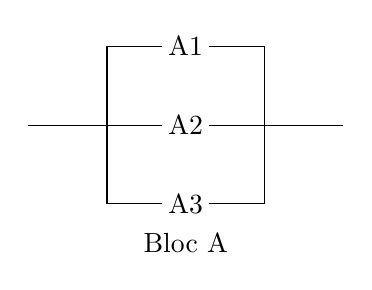
\begin{tikzpicture}	
		% bandes extérieures
		\draw (0,0)--(1,0);
            \draw (3,0)--(4,0);

            % étiquette éléments
		\node at (2,1) {A1};
		\node at (2,0) {A2};
            \node at (2,-1) {A3};
            
            % vers les étiquettes
            \draw (1,1) -- (1.7,1); %vers A1
            \draw (1,0) -- (1.7,0); %vers A2
            \draw (1,-1) -- (1.7,-1); %vers A3
            
            % à partir des étiquettes
            \draw (2.3,1) -- (3,1); %de A1
            \draw (2.3,0) -- (3,0); %de A2
            \draw (2.3,-1) -- (3,-1); %de A3

            %premiers verticaux
            \draw (1,0) -- (1,1); % A1
            \draw (1,0) -- (1,-1); % A3

            %deuxièmes verticaux
            \draw (3,0) -- (3,1); % A1
            \draw (3,0) -- (3,-1); % A3
		
		\node at (2,-1.5) {Bloc A};
    \end{tikzpicture} \end{center}
\end{figure}
	
 Le bloc A contient trois éléments. Nous avons que
\begin{itemize}
    \item L'élément A1 fonctionne avec une probabilité de 0,60.
    \item L'élément A2 fonctionne avec une probabilité de 0,50.
    \item L'élément A3 fonctionne avec une probabilité de 0,60.
\end{itemize}
Pour que le montage fonctionne, au moins un élément du bloc A doit fonctionner. Les éléments d'un bloc fonctionnent de façon indépendante.
	
\vspace{0,3cm}

 Quelle est la probabilité que le montage ne fonctionne pas? 


 \begin{oneparcheckboxes}
		\choice 0,08
		\correctchoice 0,92
		\choice 0,18 
		\choice 0,82
		\choice 0,63
\end{oneparcheckboxes}

\begin{solution}
On cherche la loi de
		\begin{eqnarray*}
			{X}_2|{X}_1=101 &\sim& N\left(\mu_2 +\rho\, \sigma_2\, \left(\frac{x_1-\mu_1}{\sigma_1}\right),\sigma_2^2 \,\left(1-\rho_2^2\right)\right)\\
			&\sim& N\left(84 +0.8\times 5\times \left(\frac{101-92}{3}\right),25 \,\left(1-0.8^2\right)\right)\\
			&\sim& N\left(96, 9 \right)
	\end{eqnarray*}
\end{solution}

\vspace{1cm}
\newpage
.
\newpage
\question[3] Une personne a $n$ clés sur son porte-clés.
Parmi ces $n$ clés, $k$ clés déverrouillent une même serrure. 
La personne tente de déverrouiller cette serrure en utilisant une succession de clés, avec remise, c'est-à-dire qu'après avoir tenté avec une clé qui ne fonctionne pas, la clé est remise dans le lot.
On note $X$ la variable aléatoire du nombre de clés testées avant que la serrure soit déverrouillée.
Que vaut $P(X=k)$?

\begin{oneparcheckboxes}
    \choice $\displaystyle \left(\frac{n-k}{n}\right)^{k-1}\frac{k}{n}$
    \choice $\displaystyle \binom{n}{k}\left(\frac{k}{n}\right)^{k}\left(1-\frac{k}{n}\right)^{n-k}$
    \correctchoice $\displaystyle \binom{k-1}{n-1}\left(\frac{k}{n}\right)^{n}\left(1-\frac{k}{n}\right)^{n-k}$
    \choice $\displaystyle \frac{k}{n}$
\end{oneparcheckboxes}

\vspace{0.5cm}

\question\label{pa} Soient $A$, $B$ et $C$ trois événements avec $P(A)=0,5$, $P(B)=0,5$, $P(C)=0,2$, $P(A\cap B)=0,25$. Nous avons aussi que $C$ est indépendant de l'événement $A$ et de l'événement $B$. Dites si chacun des énoncés ci-dessous est vrai ou faux. Votre réponse doit être justifiée en mots ou par des calculs. Un vrai ou faux sans justification n'aura aucun point.

\vspace{0.5cm}
\begin{parts}

\part[3] Les événements $A$ et $B$ sont indépendants.

     \begin{oneparcheckboxes}
		\choice VRAI
		\correctchoice FAUX
\end{oneparcheckboxes}\\
{\bf Justification:}
\vspace{4cm}

\part[3] $P(A\cup C)= 0,6$.

\begin{oneparcheckboxes}
		\choice VRAI
		\correctchoice FAUX
\end{oneparcheckboxes}\\
{\bf Justification:}
\vspace{4cm}
\part[3] Les événements $A$ et $B$ forment une partition de l'espace échantillonnal.

     \begin{oneparcheckboxes}
		\choice VRAI
		\correctchoice FAUX
\end{oneparcheckboxes}\\
{\bf Justification:}
\end{parts}


\newpage . \newpage

\question 
Soit la fonction $f$ définie sur $\mathbb{R}$ par 
\begin{align*}
f(x)= \left\{
\begin{tabular}{l l}
$c e^{x}$,&\mbox{si $x<0$},\\
$0$,& \mbox{sinon},
\end{tabular}
\right.
\end{align*}
où $c\in\mathbb{R}$ est une constante donnée. 

\vspace{0.2cm}
\begin{parts}
    
\part[3] Quelle doit être la valeur de la constante $c$ pour que $f$ soit une densité de probabilité d'une certaine variable aléatoire~$X$?
\vspace{4cm}


\part[3] Déterminer la fonction de répartition de $X$. \textit{Si vous n'avez pas trouvé «$c$» à la question} (a), \textit{vous pouvez exprimer la répartition avec «$c$».}
\vspace{4cm}




\part[5] Calculer l'espérance de $X$. \textit{Si vous n'avez pas trouvé «$c$» à la question} (a), \textit{vous pouvez exprimer l'espérance avec «$c$».}
\vspace{4cm}




\end{parts}

\newpage . \newpage
\question
La lune suscite un grand intérêt pour les pêcheurs car la qualité de la pêche dépend directement des différentes phases lunaires. Un pêcheur a remarqué les faits suivants pour chaque période d'une heure de pêche:

\begin{itemize}
    \item Lorsque la lune est croissante, la probabilité de pêcher au moins un poisson est de cinq sur sept;
    \item Lorsque la lune est décroissante, la probabilité de ne pêcher aucun poisson est de deux sur cinq.
\end{itemize}
La lune est considérée la moitié du temps comme croissante, et l'autre moitié comme décroissante.
\vspace{1cm}

\begin{parts}
    \part[3] Quelle est la probabilité qu'en pêchant une heure, le pêcheur pêche au moins un poisson?
\vspace{4cm}

\part[3] Si le pecheur ne pêche aucun poisson après une heure de pêche, quelle est la probabilité que la lune soit croissante?
\vspace{4cm}

\part[3] Si, en période de lune croissante, il pêche trois heures de suite, quelle est la probabilité qu'il ne pêche aucun poisson?
\vspace{4cm}

\part[3] Si, en période de lune décroissante, il pêche aussi trois heures de suite, quelle est la probabilité qu'il pêche au moins un poisson ?
\end{parts}


\newpage . \newpage
\question[10] \label{CDF} La variable aléatoire $X$ suit une loi normale d'espérance $\mu$ et de variance $\mu^4$.

Sachant que $P(X\leq 0)= 0,84134$ et que $P(X>1)=0,002275$, que vaut $\mu_X$?

\newpage . \newpage
\question
L'examen A et l'examen B servent pour la classification à un même emploi. 
Nous savons que les notes de ces deux examens suivent des lois normales d'espérance $\mu_{A}=1100$ et $\mu_{B}=21$, respectivement, de variance $\sigma^2_{A}=40\ 000$ et $\sigma^2_{B}=36$, respectivement et de fonctions de répartition $F_A$ et $F_B$, respectivement.
Nous établissons le pointage d'un candidat par la probabilité d'obtenir une note inférieure ou égale à la note du candidat en question (donc en évaluant $F_A(a)$ ou $F_B(b)$, pour un candidat ayant obtenu $a$ à l'examen A ou $b$ à l'examen B). 

\begin{parts}
    \part[4] Sophie a eu une note de 1300 à l'examen A alors que Maxime a eu une note de 24 à l'examen B. Lequel des deux a un meilleur pointage?
\vspace{8cm}

\part[4] Quelle note aurait dû avoir Sophie afin d'obtenir le même pointage que Maxime?
\end{parts}

\newpage . \newpage
  \question Soit $X$ et $Y$, deux variables aléatoires.
Voici le tableau qui représente la fonction de masse conjointe de $(X, Y)$ où les lettres $\boldsymbol{a},\hdots,\boldsymbol{i}$ sont des probabilités.

\begin{center}
\large{
\begin{tabular}{cc|ccc|c}
$p(x,y)$    &       &               & $x$ &     &\\
            &       & $0$           & $1$ & $2$ & $p_Y(y)$\\ 
 \hline
            & $-1$ & $\sfrac{1}{16}$ & $\boldsymbol{a}$  & $\sfrac{1}{16}$ &$\sfrac{4}{16}$\\

 $y$        & $0$   &     $\boldsymbol{b}$          &$\sfrac{3}{16}$   &  $\boldsymbol{c}$& $\boldsymbol{d}$\\
            & $1$   &       $\boldsymbol{e}$        &  $0$& $\boldsymbol{f}$ & $\boldsymbol{g}$\\
\hline
&$p_X(x)$   & $\sfrac{4}{16}$  &$\boldsymbol{h}$ &$\boldsymbol{i}$& \\
\end{tabular}
}
 \end{center}

    
Nous avons aussi les deux informations suivantes:
\begin{itemize}
    \item $P(X+Y=1)=\displaystyle \sfrac{6}{16}$
    \item $E(Y)=0$
\end{itemize}

\vspace{0.5cm}

\begin{parts}
    \part[9] Que valent les probabilités suivantes? Vous devez justifier vos résultats.

    \begin{enumerate}[label = {}]
        \item $\boldsymbol{a}=$
        \vspace{2cm}
        \item $\boldsymbol{d}=$
        \vspace{2cm}
        \item $\boldsymbol{e}=$
        \vspace{2cm}

    \end{enumerate}
    
    \part[4] Est-ce que $X$ et $Y$ sont indépendentes ? Justifier votre réponse.
\vspace{5cm}
    \part[4] Calculer $\mathbb{E}[Y|X=1]$. \textit{Si vous n'avez pas trouvé $a$, $d$ et/ou $e$, vous pouvez exprimer votre réponse en fonction d'une ou plusieurs de ces inconnues.}
\end{parts}
\newpage . \newpage
\question[]\label{micro}
Dans un laboratoire de microtechnique, Audrey et Vincent ont étudié le temps de réaction (en millisecondes) d'un certain type de détecteur de mouvements. Les 21 valeurs suivantes sont des temps de réaction collectés au cours d'une journée:

\begin{center}
\begin{tabular}{  c c c c c c c c }
111  &111  &111  &112  &113  &113  &113 \\
113 &115  &115  &115  &115 &115 & 116 \\
116 & 118 & 118 & 119 & 125 &125 & 128\\
\end{tabular}
\end{center}

Le diagramme en boîte ci-dessous a été tracé à partir de ces résultats. Il manque toutefois quelque chose à ce diagramme (il ne s'agit pas d'un titre ou de noms d'axes).

\medskip

\begin{parts}
\part[3] Ajoutez \textbf{sur le diagramme} l'élément manquant et dites ce que vous avez fait (ceci \textit{doit} inclure des calculs) sous le diagramme. Un ajout sur le diagramme sans justification n'aura aucun point.
\begin{center}
		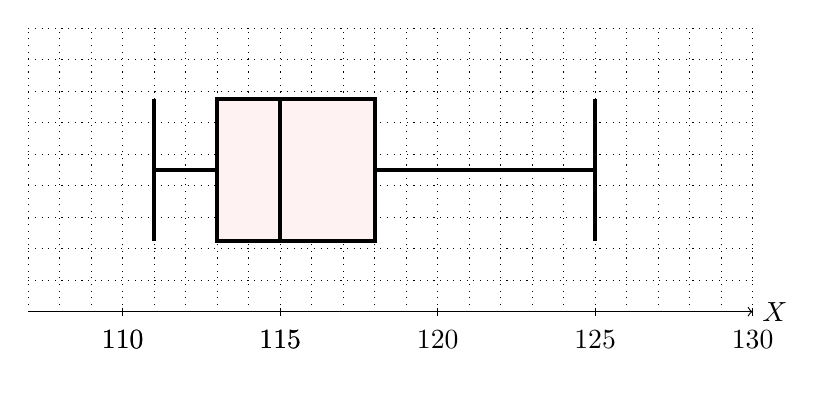
\begin{tikzpicture}[x=0.4cm,y=0.9cm]
         \draw[step=0.4cm,,dotted,color=black] (107,0) grid (130,4);
		\draw[->] (107,0) -- (130,0) node[right] {$X$} ;
		\foreach \X in {110,115,110,115,120,125,130} {
			\draw (\X,0.05cm) -- (\X,-0.05cm) node[below] {$\X\strut$};}
		\draw[ultra thick][fill=red!5] (113,1) rectangle (118,3);
  	\draw[ultra thick] (115,1) -- (115,3);

		\draw[ultra thick] (111,1) -- (111,3);
		\draw[ultra thick] (111,2) -- (113,2);
		\draw[ultra thick] (118,2) -- (125,2);
		%\draw[ultra thick] (4,1) -- (4,3);
		\draw[ultra thick] (125,1) -- (125,3);
			\end{tikzpicture}\\
	\end{center}
 \begin{solution}
     Il manque la médiane à (114 + 114) /2 = 114
 \end{solution}
\vspace{13cm}

\pagesuivante{\ref{micro}}
\newpage . \newpage
\suite{\ref{micro}}

\part[6] Nous apprenons que la plus grande observation (128) est erronée. Nous ne connaissons pas sa valeur, mais nous savons que celle-ci est plus grande que 150. Nous notons cette valeur XXX et nous savons que XXX~$>$~150. Le nouveau jeu de données est donc:

\begin{center}
\begin{tabular}{  c c c c c c c c }
111  &111  &111  &112  &113  &113  &113 \\
113 &115  &115  &115  &115 &115 & 116 \\
116 & 118 & 118 & 119 & 125 &127 & XXX\\
\end{tabular}
\end{center}

À partir de ce nouveau jeu de données, répondez aux questions suivantes. Nous nommons «jeu de données original» celui qui contient l'observation 128 et «nouveau jeu de données» celui qui contient l'observation XXX.

Déterminez si les énoncés suivants sont vrais ou faux. 

\textbf{\textit{Une bonne réponse vaut 2 points, une mauvaise réponse vaut -1 point et une réponse vide vaut 0 point, pour un total minimum de 0 point.}}

\begin{subparts}
\subpart La médiane échantillonnale du nouveau jeu de données est supérieure à celle du jeu de données original.

    \begin{oneparcheckboxes}
        \choice Vrai
        \correctchoice Faux
    \end{oneparcheckboxes}
    
\begin{solution}
    Faux
\end{solution}

\subpart La moyenne échantillonnale du nouveau jeu de données est supérieure à celle du jeu de données original.

    \begin{oneparcheckboxes}
        \correctchoice Vrai
        \choice Faux
    \end{oneparcheckboxes}
    
\begin{solution}
    Vrai
\end{solution}

\subpart La variance échantillonnale du nouveau jeu de données est supérieure à celle du jeu de données original.

    \begin{oneparcheckboxes}
        \correctchoice Vrai
        \choice Faux
    \end{oneparcheckboxes}
    
\begin{solution}
    Vrai
\end{solution}

\end{subparts}
\end{parts}

\newpage . \newpage


\question Un employé d'un centre d'appel reçoit en moyenne 8 appels par heure. Pour chacune des sous-questions de cet exercice, vous aurez 1 point si vous identifiez la bonne loi et son(ses) paramètre(s).

\begin{parts}
    \part[4] Quelle est la probabilité que l'employé reçoive 2 appels dans les 30 prochaines minutes ?
    \begin{solution}
    Processus de poisson d'intensité 1 patient / 10 minutes.\\
    $X$: nombre de patients par 30 minutes\\
    $X\sim$Poisson($\mu=1 \cdot 30 / 10$), donc $X\sim$Poisson($\mu=3$).\\
    On cherche $P(X=2) = \displaystyle\frac{3^2e^{-3}}{2!}= \frac{9e^{-3}}{2}$
    
    \end{solution}
    \vspace{5cm}
    \part[4] L'employé a reçu 3 appels dans les 7 dernières minutes. Quelle est la probabilité que le prochain appel surviennent dans 10 minutes?
    \begin{solution}
     Processus de poisson d'intensité 1 patient / 10 minutes.\\
        $Y$: temps entre deux patients\\
        $Y\sim$Exp($\frac{1}{10}$)\\
        On cherche $P(Y>12)=1-(1-e^{-12/10})=e^{-6/5}$
    \end{solution}
    \vspace{5cm}
    \part[4] L'employé a maintenant reçu 18 appels dans les 2 dernières heures. Quelle est l'espérance du temps avant que les 5 prochains appels surviennent?
    \begin{solution}
      Processus de poisson d'intensité 1 patient / 12 minutes.\\
    $W$: temps avant le 5e patient\\
    $W\sim$Gamma($5, \frac{1}{10}$)\\
    On cherche $\mathbb{E}(W)=5\cdot10=50$
    \end{solution}
\end{parts}
\newpage . \newpage
\bonusquestion[5]
Soit la variable aléatoire $X$ dont la fonction de répartition est donnée par

\begin{align*}
F_X(x)= \left\{
\begin{tabular}{l l}
$1- e^{-x}$,&\mbox{si $0\leq x$},\\
$0$,& \mbox{sinon},
\end{tabular}
\right.
\end{align*}
et la variable aléatoire $Y=aX+b$, où $a,b\in\mathbb{R}$.
Quelle est la fonction de répartition de Y?



\end{questions}
\newpage
.


\end{document} 

1=2\times 0,84134-1=0,6826,
\end{align*}
où $\Phi$ est la fonction de répartition de la loi normale centrée réduite.

\end{solution}

\vspace{6cm}

\part[6] On souhaite régler la machine de manière à obtenir qu'une tablette choisie au hasard soit mise sur le marché avec une une probabilité de $\mathbb{P}(198 \le X \le 202) = 0{,}95$. Déterminez la valeur de l'écart-type $\sigma$ qui permet d’atteindre cet objectif.

\medskip

\begin{solution}
    
En utilisant l'expression obtenue précédemment,
\[
2\Phi\!\Big(\frac{2}{\sigma}\Big)-1 = 0{,}95, 
\]
avec $\Phi\!\Big(\frac{2}{\sigma}\Big)=
\mathbb{P}\!\left(Z \le \frac{2}{\sigma}\right)$. On en déduit
\[
\Phi\!\Big(\frac{2}{\sigma}\Big) = 0{,}975.
\]
Soit $z_{0.975} = \Phi^{-1}(0.975)$ le quantile $97{,}5\%$ de la loi normale centrée réduite. On connaît la valeur numérique
\[
z_{0.975}\approx 1{,}959963984540054.
\]
Ainsi
\[
\frac{2}{\sigma} = z_{0.975}
\quad\Longrightarrow\quad
\sigma = \frac{2}{z_{0.975}} \approx \frac{2}{1{,}959963984540054}
\approx 1{,}02043\ \text{grammes}.
\]
On peut donc régler la machine pour obtenir un écart-type d'environ \(\sigma\approx 1{,}0204\) g, ce qui garantit que \(95\%\) des tablettes ont une masse entre 198 g et 202 g. \end{solution}

\end{parts}
\pageblanche
%TCL-Ahmed
\question[]
On effectue un contrôle de fabrication sur des pièces dont une proportion $p=0.02$ est défectueuse. 

\begin{parts}
    \part[4] On contrôle un lot de $1000$ pièces: Soit $X$ la variable aléatoire : « nombre de pièces défectueuses parmi $1000$ ». 
    Quelle est la loi de $X$ ? 

    \begin{solution}
        
    
    On a $X \sim \text{Binomiale}(n=1000, p=0.02)$. \\
    Espérance : $\mathbb{E}[X] = np = 1000 \times 0.02 = 20$. \\
    Variance : $\mathrm{Var}(X) = np(1-p) = 1000 \times 0.02 \times 0.98 = 19.6$. \\
    Écart-type : $\sigma_X = \sqrt{19.6} \approx 4.43$.
    \end{solution}

\vspace{10cm}
    \part[4] En approximant cette loi par celle d’une loi normale, calculez la probabilité que $X$ soit compris entre $18$ et $22$. 

    \begin{solution}
        
    
    Approximation normale : $X \approx \mathcal{N}(20, 19.6)$. \\
    Sans correction de continuité : \\
    $\mathbb{P}(18 \leq X \leq 22) \approx \mathbb{P}\!\left(\frac{18-20}{4.43} \leq Z \leq \frac{22-20}{4.43}\right) = \mathbb{P}(-0.45 \leq Z \leq 0.45)\approx 2\Phi(0.45)-1 \approx 0.349.$ \\
    Avec correction de continuité : \\
    $\mathbb{P}(18 \leq X \leq 22) \approx \mathbb{P}\!\left(\frac{17.5-20}{4.43} \leq Z \leq \frac{22.5-20}{4.43}\right) = \mathbb{P}(-0.56 \leq Z \leq 0.56)\approx 2\Phi(0.56)-1 \approx 0.428.$
    \end{solution}
\end{parts}








\pageblanche

\question[3] 
\begin{center}
    

\begin{tikzpicture}[scale=1.1]

%--- positions des sommets principaux
\coordinate (A) at (-1,2.2);

\coordinate (B) at (-5,0.0);
\coordinate (C) at (-1.9,0.6);
\coordinate (D) at (1.8,0.6);
\coordinate (E) at (6.1,0.9);

\coordinate (F) at (-6,-1);
\coordinate (G) at (-5,-1.1);
\coordinate (H) at (-4,-1);

\coordinate (I) at (0,-2.1);

\coordinate (J) at (3.3,-1.4);

\coordinate (K) at (5.1,-1.4);
\coordinate (L) at (6.1,-1.4);
\coordinate (M) at (7.1,-1.4);


%--- étiquettes
\node[pt,above] at (A) {A};
\node[pt,left]  at (B) {B};

\node[pt,above] at (C) {C};
\node[pt,above] at (D) {D};
\node[pt,above right] at (E) {E};

\node[pt,below] at (F) {F};
\node[pt,below] at (G) {G};
\node[pt,below] at (H) {H};

\node[pt,below] at (I) {I};
\node[pt,above left] at (J) {J};
\node[pt,below] at (K) {K};
\node[pt,below] at (L) {L};
\node[pt,below] at (M) {M};

%--- polygonal / intérieur (A-C-X-D-A)
\draw[mid arrow] (A) -- (B);
\draw[mid arrow] (A) -- (C);
\draw[mid arrow] (A) -- (D);
\draw[mid arrow] (A) -- (E);


\draw[mid arrow] (B) -- (F);
\draw[mid arrow] (B) -- (G);
\draw[mid arrow] (B) -- (H);

\draw[mid arrow] (B) -- (I);

\draw[mid arrow] (C) -- (I);

\draw[mid arrow] (D) -- (I);

\draw[mid arrow] (E) -- (I);
\draw[mid arrow] (E) -- (J);
\draw[mid arrow] (E) -- (K);
\draw[mid arrow] (E) -- (L);
\draw[mid arrow] (E) -- (M);

\draw[mid arrow] (J) -- (I);




%--- petits cercles ouverts sur la chaîne Bmid arrowA


%--- points visibles A,B,C,D,E,X
\node[dot] at (A) {};
\node[dot] at (B) {};
\node[dot] at (C) {};
\node[dot] at (D) {};
\node[dot] at (E) {};
\node[dot] at (F) {};
\node[dot] at (G) {};
\node[dot] at (H) {};
\node[dot] at (I) {};
\node[dot] at (J) {};
\node[dot] at (K) {};
\node[dot] at (L) {};
\node[dot] at (M) {};

\end{tikzpicture}
\end{center}

Une randonneuse part du point A en choisissant au hasard parmi les sentiers $AB$, $AC$, $AD$ et $AE$.
Elle s'arrête seulement lorsqu'elle est arrivée à $F,G,H,I,K,L$ ou $M$.
Quelle est la probabilité qu'elle ne s'arrête pas au point $M$?

\vspace{0.25cm}
\begin{checkboxes}
    \choice 1/7
    \choice 1/8
    \choice 1/5
    \choice 1/20
    \choice 1/24
    \choice 1/16
    \choice 6/7
    \choice 7/8
    \choice 4/5
    \correctchoice 19/20
    \choice 23/24
    \choice 15/16
    \choice 10/11
\end{checkboxes}

\vspace{0.5cm}
\question[3]\label{module1_1}  
On nous donne les probabilités suivantes:
\[
\begin{aligned}
    & P(A) = 0,45 \\
    & P(B) = 0,25 \\
    & P(C) = 0,30 \\
    & P(C|A) = 0,30 \\
    & P(C|B) = 0,30 \\
    & P(A \cap B) = 0,05 \\
\end{aligned}
\]

Cochez tous les énoncés qui sont \textbf{vrais}, sachant que deux énoncés sont vrais. \textit{Chaque énoncé qui est coché alors qu'il ne devrait pas l'être annule les points d'un élément coché qui devrait l'être.}
\begin{checkboxes}
\choice $P(A \cup B) = 0,70$
\correctchoice $ P(A \cap \overline{B}) = 0,40 $
\choice $ P(A \cap C) = 0,1575 $
\choice $ P(A \cup C) = 0,75 $
\choice $A$ et $B$ sont indépendants
\correctchoice $A$ et $C$ sont indépendants
\choice Comme $B$ et $C$ sont indépendants, ils sont mutuellement exclusifs
\end{checkboxes}

\pageblanche

\question Soit l'histogramme suivant:

\begin{center}
    
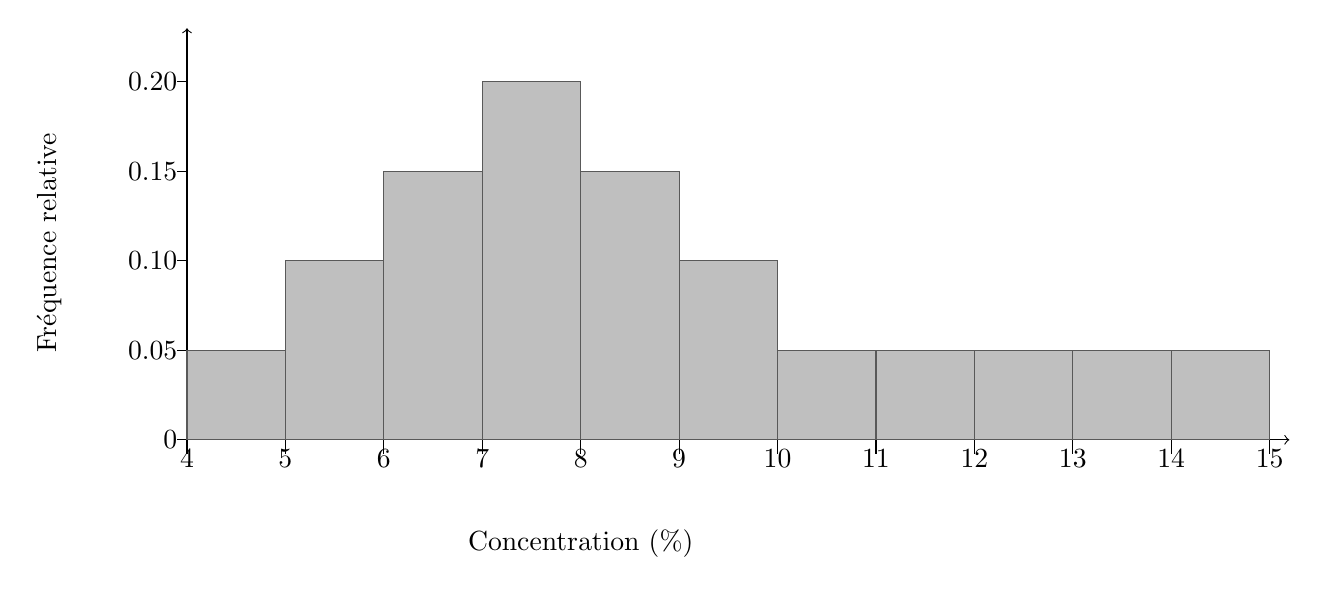
\begin{tikzpicture}[x=1.25cm, y=22.727cm] % 10 cm de large (8 unités) et 5 cm de haut (0.22 unités)
  % Axes
  \draw[->] (4,0) -- (15.2,0);
  \draw[->] (4,0) -- (4,0.23);

  % Graduations en x
  \foreach \x in {4,...,15} {
    \draw (\x,0) -- (\x,-0.008);
    \node[below] at (\x,0) {\x};
  }

  % Graduations en y
  \foreach \y/\lab in {0/0,0.05/0.05,0.10/0.10,0.15/0.15,0.20/0.20}{
    \draw (4,\y) -- (3.9,\y);
    \node[left] at (4,\y) {\lab};
  }

  % Titres d'axes
  \node[below] at (8,-0.045) {Concentration (\%)};
  \node[rotate=90] at (2.6,0.11) {Fréquence relative};

  % Barres : classes [4,5[, [5,6[, ..., [11,12[
  \foreach \x/\h in {4/0.05,5/0.1,6/0.15,7/0.20,8/0.15,9/0.1,10/0.05,11/0.05,12/0.05,13/0.05,14/0.05} {
    \fill[gray!50] (\x,0) rectangle (\x+1,\h);
    \draw[gray!70!black] (\x,0) rectangle (\x+1,\h);
  }
\end{tikzpicture}
\end{center}

Déterminez si les énoncés suivants sont vrais ou faux. 

\textbf{\textit{Une bonne réponse vaut 1 points, une mauvaise réponse vaut -1 point et une réponse vide vaut 0 point, pour un total minimum de 0 point.}}

\vspace{0.5cm}
\begin{parts}
    \part[2] Il est impossible de donner la taille de l'échantillon qui a servi à tracer cet histogramme avec l'information donnée.

    \begin{oneparcheckboxes}
        \correctchoice Vrai
        \choice Faux
    \end{oneparcheckboxes}

\vspace{0.25cm}
\part[2] Cet histogramme est typique de données provenant d'une distribution où la moyenne est supérieure à la médiane.

    \begin{oneparcheckboxes}
        \correctchoice Vrai
        \choice Faux
    \end{oneparcheckboxes}

\vspace{0.25cm}
\part[2] L'écart interquartile vaut au moins 5,5.

    \begin{oneparcheckboxes}
        \choice Vrai
        \correctchoice Faux
    \end{oneparcheckboxes}

    \vspace{0.25cm}

\part[2] La médiane échantillonnale est entre 7\% et 9\%, inclusivement.

    \begin{oneparcheckboxes}
        \correctchoice Vrai
        \choice Faux
    \end{oneparcheckboxes}

\part[2] L'écart-type échantillonnal est de 11\%.

    \begin{oneparcheckboxes}
        \choice Vrai
        \correctchoice Faux
    \end{oneparcheckboxes}
    
    \end{parts}

\vspace{0.25cm}
\question[3] Soit $A$ et $B$, deux événements de $\mathcal{U}$, avec $P(A)>0$ et $P(B)>0$.Quel énoncé est \textbf{toujours} vrai?

\vspace{0.25cm}
\begin{checkboxes}
    \choice Si $P(A)+P(B)=1$, $A$ et $B$ forment une partition de $\mathcal{U}$.
    \choice Si $P(A\cap B)=0$, $A$ et $B$ sont indépendants.
    \correctchoice Si $A$ et $B$ sont indépendants, ils ne sont pas mutuellement exclusifs.
    \choice Si $A\subset B$, le fait que $B$ se réalise implique que $A$ se réalise.
\end{checkboxes}
    \pageblanche
    
\question 

Supposons que dans la population, il y a $51\%$ d'hommes ($H$) et $49\%$ de femmes ($F$), et que le daltonisme ($D$) est réparti de cette façon:

\begin{table}[h]
    \centering
    \begin{tabular}{l|c|c}
    \hline \hline
        & Hommes ($H$) & Femmes ($F$) \\
    \hline
        Daltoniens ($D$) & 0,04 & $XXX$ \\ 
        Non daltoniens ($\overline{D}$) &0,47 & $YYY$ \\
        \hline

        \hline
    \end{tabular}
\end{table}

Nous savons que la probabilité qu'une femme choisie au hasard soit daltonienne est de $\frac{1}{245}$.

\begin{parts}
    \part[6]Quelle est la probabilité qu'une personne choisie au hasard soit une femme et soit non daltonienne?
\begin{solution}
    Nous savons que $P(D|F)=\frac{1}{245}$. Nous avons donc 
    \begin{align*}
        P(D|F)&= \frac{P(D\cap F)}{P(F)}\\
        \frac{1}{245}&= \frac{P(D\cap F)}{0,49}\\
        0,49 *\frac{1}{245}&=P(D\cap F)\\
        P(D\cap F)&=\frac{1}{500}
    \end{align*}
    Nous savons donc que $XXX=\frac{1}{500}$. Comme nous avons que $0,04+0,47+XXX+YYY=1$, nous déduisons $YYY=0,488$
\end{solution}
    \vspace{10cm}
    \part[3] $H$ et $F$ sont indépendants.

     \begin{oneparcheckboxes}
		\choice VRAI
		\correctchoice FAUX
\end{oneparcheckboxes}\\
{\bf Justification:}
\vspace{4cm}
        \part[3] $H$ et $D$ sont indépendants.

     \begin{oneparcheckboxes}
		\choice VRAI
		\correctchoice FAUX
\end{oneparcheckboxes}\\
{\bf Justification:}
\end{parts}


\pageblanche


\question Soit la variable aléatoire discrète $X$ dont la fonction de probabilité est donnée dans le tableau suivant:

\begin{table}[h]
    \centering
        \begingroup
\setlength{\tabcolsep}{10pt}    % espace entre colonnes
\renewcommand{\arraystretch}{1.5}% espace entre lignes
    \begin{tabular}{|c|c|c|c|c|c|c|c|}
    \hline
        $x$ & 1 & 2 & 3 & 5 & 8 & 13 & 21  \\
        \hline
        $p(x)$ & 0,05 & 0,1 & 0,01 & 0,3 & 0,5 & 0,01 &0,03\\
        \hline
    \end{tabular}
    \endgroup
    \end{table}
Nous avons $p(x)=0$ pour tous les $x$ qui ne sont pas donnés dans le tableau.

\begin{parts}
    \part[4] Remplissez le tableau suivant.

    \begin{table}[h]
    \centering
    \begingroup
\setlength{\tabcolsep}{16pt}    % espace entre colonnes
\renewcommand{\arraystretch}{2.5}% espace entre lignes

    \begin{tabular}{|c|c|c|c|c|c|c|c|c|c|}
    \hline
        $x$ & 0 & 1 & 2 & 3 & 5 & 8 & 13 & 21 & 30  \\
        \hline
        F(x) & &  &  &  &  &  & & &\\
        \hline
    \end{tabular}
    \endgroup

    \end{table}

    \part[4] Calculez l'espérance de $X$.

    \begin{solution}
        \begin{align*}
            E(X)&=\sum_{x\in \mathbb{R}_X}xp(x)\\
            &= 1 *0,05 + 2 *0,1+\hdots+21*0,03\\
            &=6,54
        \end{align*}
    \end{solution}

    \vspace{8cm}
    \part[4] Soit $W$ une variable aléatoire qui vaut $2$ si le résultat de $X$ est pair et qui vaut $1$ si celui-ci est impair. 
    Donnez la fonction de probabilité de $W$. 

    \begin{solution}
        $$p(w)=\left\{\begin{array}{ll}
0,4, & w=1,\\
0,6, & w=2,\\
0, & \text{sinon}.
\end{array}\right.$$
    \end{solution}
\end{parts}
\pageblanche

\question\label{repartition} Soit la variable aléatoire $X$ dont la fonction de répartition est donnée par:

$$F(x)=\left\{\begin{array}{ll}
0, & x<0,\\
x^2, & 0\leq x \leq 1,\\
1, & x>1.
\end{array}\right.$$
\begin{parts}

    \part[3] Quelle est la valeur de $m$, la médiane de $X$? C'est-à-dire, trouvez $m$, tel que $P(X<m)=0,5$.
    
\begin{solution}
    \begin{align*}
        0,5&=P(X<m)\\
        &= F(m)\\
        &= m^2\\
        \sqrt{0,5}&=m\\
        m&=  \sqrt{0,5}=\frac{\sqrt{2}}{2}=0,707    
    \end{align*}
\end{solution}
    \vspace{7cm}
    \part[4] Calculez la probabilité que $X$ soit compris entre 0,2 et 0,3, sachant que $X$ est supérieur à 0,1.
\begin{solution}
    \begin{align*}
        P(0,2<X<0,3|X>0,1)&=\frac{P(0,2<X<0,3\cap X>0,1)}{P(X>0,1)}\\
        &= \frac{P(0,2<X<0,3)}{P(X>0,1)}\\
        &= \frac{F(0,3)-F(0,2)}{1-F(0,1)}\\
        &= \frac{0,09-0,04}{0,99}\\
        &= \frac{5}{99}=0,0505
    \end{align*}
\end{solution}
\vfill
    \pagesuivante{\ref{repartition}}
\pageblanche
\suite{\ref{repartition}}

    \part[3] Donnez la fonction de densité de $X$.
\begin{solution}
    $$\displaystyle f(x)=\frac{dF(x)}{dx}=\left\{\begin{array}{ll}
\displaystyle\frac{d}{dx}0, & x<0,\\
\displaystyle\frac{d}{dx}x^2, & 0\leq x \leq 1,\\
\displaystyle\frac{d}{dx}1, & x>1.
\end{array}\right.$$

    $$\displaystyle f(x)=\left\{\begin{array}{ll}
2x, & 0\leq x \leq 1,\\
0, & \text{sinon}.
\end{array}\right.$$
\end{solution}
    
\end{parts}
\pageblanche
\end{questions}
\end{document} 
